\begin{figure*}[t]
\centering
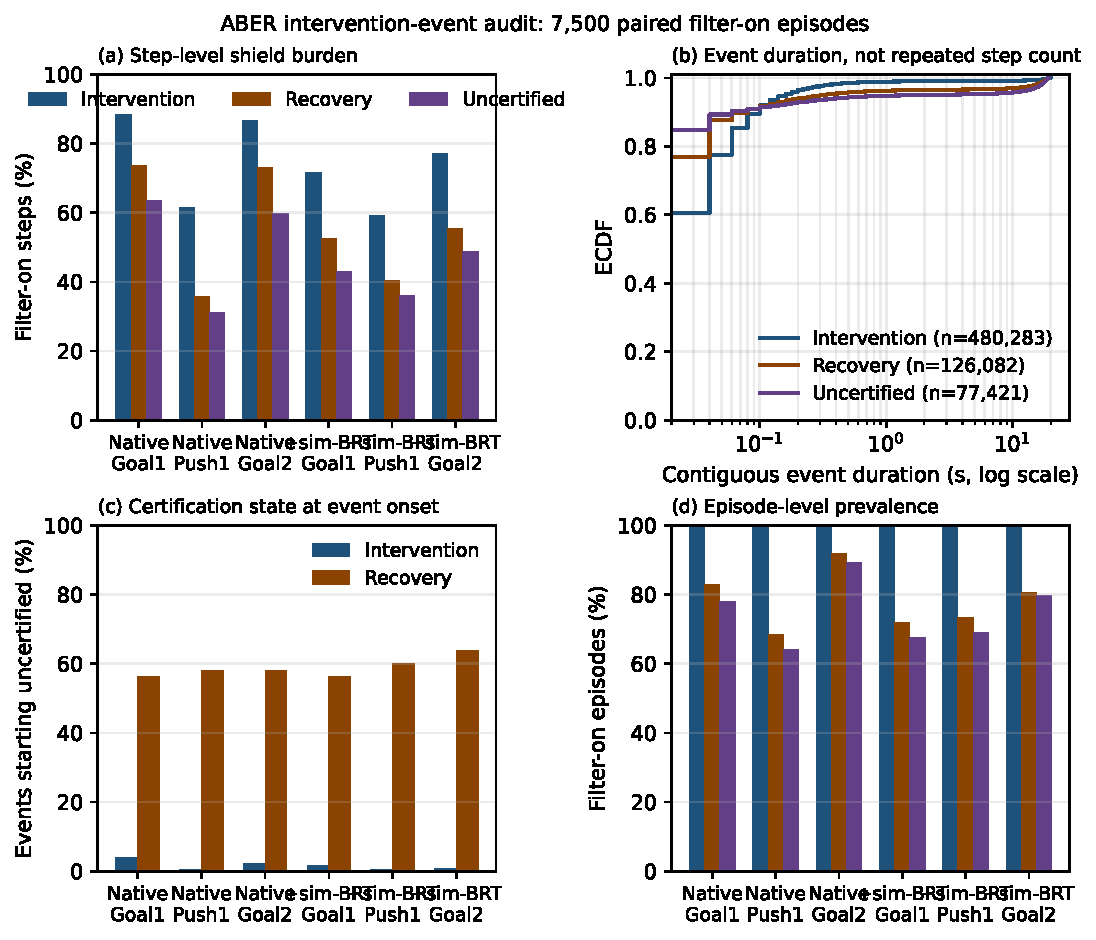
\includegraphics[width=\textwidth]{../figures/supplement/aber_intervention_event_audit.pdf}
\caption{Event-level reconstruction over all 7,500 filter-on episodes.
An event is a maximal contiguous run within one episode. Most interventions
are one-step corrections, but a small tail of long recovery/uncertified runs
dominates time under intervention; overlapping step rates in (a) are therefore
not independent categories.}
\label{fig:eventaudit}
\end{figure*}

\paragraph{Where intervention time comes from.}
The 6,485,664 filter-on steps contain 480,283 intervention events. Although
60.47\% last one step and the median is 0.02~s, the 0.98\% lasting at least
100 steps contribute 76.22\% of all intervention steps. Every one of the
2,972,091 uncertified steps is also a recovery step; 85.41\% of recovery time
is uncertified. Thus the primary efficiency bottleneck is entry into, and
long dwell within, the uncertified recovery regime, not merely frequent
one-step clipping. Debouncing can reduce switching but cannot recover most
lost task time without a separately certified directional transition model.
